\chapter{Pruebas}

En esta sección se abordarán las distintas tareas relacionadas las diferentes pruebas realizadas para asegurar la calidad del producto final antes de su entrega. El objetivo del proceso de pruebas es la verificación del software; es necesario poner a prueba el comportamiento del software para identificar situaciones en las que no se obtengan los resultados esperados.

\section{Integración continua en el repositorio}

Todas estas pruebas se han ido realizando cada vez que se actualizaba el repositorio del proyecto en GitHub. Para ello, se ha usado Travis\footnote{https://travis-ci.org/}, un sistema que permite la integración continua en el repositorio. Una vez enlazado Travis con el repositorio, la realización de test es un proceso automático que se realizará siempre.

Gracias a esta herramienta libre, se puede comprobar en cualquier momento si el software se encuentra validado o no. En el caso de que el test falle, Travis notifica dónde está el error. 

Travis necesita de un archivo de configuración \textit{.travis.yml}\footnote{https://github.com/guillesiesta/ProjectX/blob/master/.travis.yml} para el arranque, creando una máquina virtual que simulará el sistema y comenzará a examinar los cambios realizados. En este caso concreto, para realizar los tests del  el módulo de la API(Python) y de  la interfaz(Javascript), es necesario crear el archivo tal y como se muestra en la figura\ref{fig::travis}.

\begin{figure}[htbp]
    \centerline{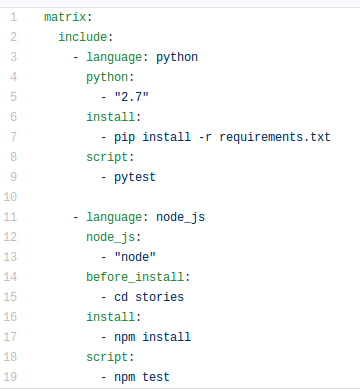
\includegraphics[width=8cm]{figuras/travis.png}}
    \caption{Archivo .travis.yml del repositorio en GitHub}
    \label{fig::travis}
\end{figure}

\section{Pruebas en \textit{back-end} - API}

Para el correcto funcionamiento de la API se ha usado la librería Pytest\footnote{https://docs.pytest.org/en/latest/} y su plugin para flask\footnote{https://pytest-flask.readthedocs.io/en/latest/}.

Esta herramienta permite la realización de tests unitarios. Para cada función de la API se ha realizado el siguiente testeo:

\begin{itemize}
    \item \textbf{all\_stories\_titulo()}. Se cuentan todas las historias existentes en la base de datos y se guarda esa cantidad. Se añade una historia y se comprueba que las historias existentes son la cantidad anterior más 1.
     \item \textbf{user\_stories\_titulo()}. Se crea un acertijo y un usuario. Se crea la relación (usuario)-[escribe]-(acertijo) y se comprueba que la historia introducida existe y está escrita por ese usuario.
     \item \textbf{soluciones\_por\_titulo()}.Se crea un acertijo y un usuario. Se crea la relación (usuario)-[propone solución]-(acertijo) y se comprueba que esa solución para ese acertijo existe.
     \item \textbf{enviar\_comentario()}. Se crea un acertijo y un usuario. Se crea la relación (usuario)-[propone solución]-(acertijo) y se comprueba que esa solución propuesta ha sido añadida en el sistema.
     \item \textbf{enviar\_storie()}. Se crea un acertijo y un usuario, se crea la relación (usuario)-[escribe]-(acertijo), y se comprueba que ese acertijo tiene todos los campos iguales que el acertijo creado.
     \item \textbf{cambiar\_puntuacion()}. Se crea un acertijo y un usuario. Se crea la relación (usuario)-[propone solución]-(acertijo). Se cambia la puntuación y se comprueba que la puntuación para esa solución propuesta ha sido modificada.
     \item \textbf{acertijo\_por\_titulo()}.Se crea un acertijo y se comprueba que, buscándolo en la base de datos por su título, éste existe.
     \item \textbf{storie\_por\_titulo()}. Se crea un acertijo y se comprueba que, buscándolo en la base da datos por su título, la solución a él existe.
     \item \textbf{todo\_por\_titulo()}. Se crea un acertijo y se comprueba que, a través de su título, se busca en la base de datos y devuelvo todos sus atributos.
     \item \textbf{login()}. Se crea un usuario en el sistema con nombre y contraseña y se comprueba que éste ha sido añadido al sistema correctamente.
\end{itemize}

Se puede acceder al código de todos los tests definidos en el repositorio de GitHub de la aplicación\footnote{https://github.com/guillesiesta/ProjectX/blob/master/stories/test\_storie.py}. 

\section{Pruebas en \textit{front-end}}

Para testear la interfaz se ha usado Jest\footnote{https://jestjs.io/} junto con Enzyme\footnote{https://github.com/airbnb/enzyme}. Esta recomendación para el testeo viene dada por la propia documentación de ReactJS\cite{testreact}.

La idea principal para las pruebas es comprobar que cada componente creado en ReactJS se renderiza de manera correcta. Para ello gracias a Enzyme, se puede crear un \textit{snapshot} o instantánea de ese componente antes de renderizar, y una vez se renderice, se comprueba que el componente está creado de la manera esperada\cite{testreact2}.

Dicho de otra manera: se le dice a Jest que se quiere estar seguro de que la salida de este componente nunca debe cambiar accidentalmente y Jest, con ayuda de Enzyme la guarda en un archivo, y después comprueba que el componente no ha sido cambiado una vez se renderice.

\section{Validación}

Como forma de validación se han creado una serie de usuarios con contraseña para que quién lo desee pueda acceder a la plataforma y comprobar que puede crear un acertijo, responder los ya existentes y puntuar las propuestas de solución que le propongan.

Cada usuario tiene asignado un acertijo creado por defecto y asignado. Todas las contraseñas son iguales: 1234.

Los usuarios son:
\begin{itemize}
    \item thor
    \item tonystark
    \item hulk
    \item ultron
    \item spiderman
    \item aristoteles
    \item socrates
    \item platon
    \item descartes
    \item epicuro
\end{itemize}

Se recuerda nuevamente la dirección web de la aplicación:

\textbf{https://riddling.herokuapp.com/}

Actualmente se está llevando a cabo este proceso, sin embargo aún no se han obtenido datos suficientes como para analizar el grado de agrado o desagrado general de la aplicación para los usuarios. 